\documentclass[11pt,a4paper]{article}
\usepackage[margin=2.3cm]{geometry}
\usepackage[T1]{fontenc}
\usepackage{lmodern}
\usepackage{microtype}
\usepackage{xspace}
\usepackage{booktabs}
\usepackage{tabularx}
\usepackage{array}
\usepackage{graphicx}
\usepackage{float}
\usepackage{xcolor}
\usepackage{enumitem}
\usepackage{caption}
\usepackage{titlesec}
\usepackage{fancyhdr}
\usepackage[hidelinks]{hyperref}

\definecolor{rmblue}{HTML}{2B6CB0}
\definecolor{rmorange}{HTML}{DD6B20}
\definecolor{rmgrey}{HTML}{4A5568}

% auto-generated by make_numbers.py -- do not edit
\newcommand{\ResRawMain}{2,484\xspace}
\newcommand{\ResRawUpd}{962\xspace}
\newcommand{\ResRaw}{3,446\xspace}
\newcommand{\ResEmpty}{1\xspace}
\newcommand{\ResMojibake}{38\xspace}
\newcommand{\ResNonEn}{0\xspace}
\newcommand{\ResExactDup}{798\xspace}
\newcommand{\ResExactDupUpd}{796\xspace}
\newcommand{\ResNearDup}{8\xspace}
\newcommand{\ResShort}{27\xspace}
\newcommand{\ResLong}{27\xspace}
\newcommand{\ResIQR}{222\xspace}
\newcommand{\ResJunk}{7\xspace}
\newcommand{\ResPlow}{97\xspace}
\newcommand{\ResPhigh}{2,047\xspace}
\newcommand{\ResPII}{117\xspace}
\newcommand{\ResPIItokens}{299\xspace}
\newcommand{\ResFinal}{2,632\xspace}
\newcommand{\ResFinalMain}{2,473\xspace}
\newcommand{\ResFinalUpd}{159\xspace}
\newcommand{\ResCats}{24\xspace}
\newcommand{\JobRawLI}{33,246\xspace}
\newcommand{\JobRawRZ}{352\xspace}
\newcommand{\JobRaw}{33,598\xspace}
\newcommand{\JobEmpty}{1\xspace}
\newcommand{\JobNonEn}{23\xspace}
\newcommand{\JobExactDup}{3,236\xspace}
\newcommand{\JobNearDup}{2,087\xspace}
\newcommand{\JobShort}{280\xspace}
\newcommand{\JobLong}{283\xspace}
\newcommand{\JobIQR}{532\xspace}
\newcommand{\JobJunk}{165\xspace}
\newcommand{\JobPlow}{42\xspace}
\newcommand{\JobPhigh}{1,331\xspace}
\newcommand{\JobPII}{4,818\xspace}
\newcommand{\JobFinal}{28,086\xspace}
\newcommand{\JobFinalLI}{27,738\xspace}
\newcommand{\JobFinalRZ}{348\xspace}
\newcommand{\JobSalaryShare}{39.8\xspace}
\newcommand{\JobSenUnknown}{7,927\xspace}
\newcommand{\JobSenMissPct}{27.3\xspace}
\newcommand{\FitPairsTrain}{6,241\xspace}
\newcommand{\FitPairsTest}{1,759\xspace}
\newcommand{\EscoSkills}{13,896\xspace}
\newcommand{\EscoAlt}{99,192\xspace}
\newcommand{\RozeeQueries}{19\xspace}
\newcommand{\RozeeQueriesDefined}{33\xspace}
\newcommand{\RozeeRequests}{556\xspace}
\newcommand{\RozeeBlocked}{87\xspace}
\newcommand{\RozeeDelay}{0\xspace}
\newcommand{\SkillVocab}{1,169\xspace}
\newcommand{\TfidfVocab}{50,000\xspace}
\newcommand{\MeanSkillsRes}{7.95\xspace}
\newcommand{\MeanSkillsJob}{3.91\xspace}
\newcommand{\YearsCovRes}{95.8\xspace}
\newcommand{\YearsCovJob}{46.9\xspace}
\newcommand{\JobCatCov}{60.9\xspace}
\newcommand{\ResTrain}{1,842\xspace}
\newcommand{\ResVal}{395\xspace}
\newcommand{\ResTest}{395\xspace}
\newcommand{\JobTrain}{19,660\xspace}
\newcommand{\JobVal}{4,213\xspace}
\newcommand{\JobTest}{4,213\xspace}
\newcommand{\Pairs}{15,755\xspace}
\newcommand{\PairsPos}{7,859\xspace}
\newcommand{\PairsHard}{5,264\xspace}
\newcommand{\PairsRand}{2,632\xspace}
\newcommand{\PairsTrain}{11,052\xspace}
\newcommand{\PairsVal}{2,351\xspace}
\newcommand{\PairsTest}{2,352\xspace}
\newcommand{\CosPos}{0.12\xspace}
\newcommand{\CosHard}{0.13\xspace}
\newcommand{\CosRand}{0.03\xspace}
\newcommand{\RefYear}{2019\xspace}
\newcommand{\ImbalanceRatio}{9.91\xspace}
\newcommand{\MedWordsRes}{745\xspace}
\newcommand{\MedWordsJob}{444\xspace}
\newcommand{\SkillsUniqJobs}{2,278\xspace}
\newcommand{\SkillsUniqRes}{1,505\xspace}
\newcommand{\SkillsOverlap}{1,302\xspace}
\newcommand{\SkillsJobOnly}{976\xspace}
\newcommand{\SkillsJaccard}{0.53\xspace}
\newcommand{\TopHundredMissing}{22\xspace}
\newcommand{\AucTfidf}{0.40\xspace}
\newcommand{\AucEmb}{0.53\xspace}
\newcommand{\EmbPos}{0.48\xspace}
\newcommand{\EmbHard}{0.46\xspace}
\newcommand{\CorrYearsSalary}{0.54\xspace}
\newcommand{\CorrWordsSkillsJob}{0.48\xspace}
\newcommand{\CorrWordsSkillsRes}{0.42\xspace}
\newcommand{\RozeeMale}{7\xspace}
\newcommand{\RozeeFemale}{1\xspace}
\newcommand{\RozeeGendered}{8\xspace}
\newcommand{\RozeeTopSkills}{artificial intelligence, Python, computer science, Git, CI/CD\xspace}
\newcommand{\ResCatMin}{BPO\xspace}
\newcommand{\ResCatMinN}{22\xspace}
\newcommand{\ResCatMax}{IT\xspace}
\newcommand{\ResCatMaxN}{218\xspace}

% auto-generated by make_tables.py -- do not edit
\newcommand{\BiPreAucHard}{0.539\xspace}
\newcommand{\BiPrePthree}{0.429\xspace}
\newcommand{\BiPreAuc}{0.644\xspace}
\newcommand{\BiAucHard}{0.724\xspace}
\newcommand{\BiPthree}{0.631\xspace}
\newcommand{\BiAuc}{0.801\xspace}
\newcommand{\BiBestEpoch}{3\xspace}
\newcommand{\BiEpochs}{3\xspace}
\newcommand{\BiTriplets}{1,842\xspace}
\newcommand{\BiRuns}{5\xspace}
\newcommand{\BiBestLr}{$1\times10^{-4}$\xspace}
\newcommand{\BiBestBs}{32\xspace}
\newcommand{\BiBestLen}{256\xspace}
\newcommand{\MnALr}{$1\times10^{-3}$\xspace}
\newcommand{\MnABs}{64\xspace}
\newcommand{\MnADrop}{0.3\xspace}
\newcommand{\MnAHidden}{256\xspace}
\newcommand{\MnAEpoch}{14\xspace}
\newcommand{\MnAValAuc}{0.860\xspace}
\newcommand{\MnAParams}{412,385\xspace}
\newcommand{\MnAAblPre}{0.783\xspace}
\newcommand{\MnAAblNoFeat}{0.834\xspace}
\newcommand{\MnBLr}{$1\times10^{-3}$\xspace}
\newcommand{\MnBBs}{64\xspace}
\newcommand{\MnBDrop}{0.5\xspace}
\newcommand{\MnBHidden}{128\xspace}
\newcommand{\MnBEpoch}{26\xspace}
\newcommand{\MnBValAuc}{0.807\xspace}
\newcommand{\MnBParams}{202,273\xspace}
\newcommand{\MnBAblPre}{0.820\xspace}
\newcommand{\MnBAblNoFeat}{0.800\xspace}
\newcommand{\MnRuns}{36\xspace}
\newcommand{\ResAF}{0.784\xspace}
\newcommand{\ResAP}{0.705\xspace}
\newcommand{\ResAR}{0.883\xspace}
\newcommand{\ResAAuc}{0.862\xspace}
\newcommand{\ResAAucLo}{0.85\xspace}
\newcommand{\ResAAucHi}{0.88\xspace}
\newcommand{\ResAAtsAuc}{0.588\xspace}
\newcommand{\ResAAtsF}{0.665\xspace}
\newcommand{\ResAPreAuc}{0.661\xspace}
\newcommand{\ResABiAuc}{0.790\xspace}
\newcommand{\ResAGbAuc}{0.832\xspace}
\newcommand{\ResALrAuc}{0.808\xspace}
\newcommand{\ResAN}{2,352\xspace}
\newcommand{\ResAPosShare}{50\xspace}
\newcommand{\ResAFP}{431\xspace}
\newcommand{\ResAFN}{136\xspace}
\newcommand{\ResBF}{0.737\xspace}
\newcommand{\ResBP}{0.668\xspace}
\newcommand{\ResBR}{0.822\xspace}
\newcommand{\ResBAuc}{0.768\xspace}
\newcommand{\ResBAucLo}{0.74\xspace}
\newcommand{\ResBAucHi}{0.79\xspace}
\newcommand{\ResBAtsAuc}{0.536\xspace}
\newcommand{\ResBAtsF}{0.678\xspace}
\newcommand{\ResBPreAuc}{0.579\xspace}
\newcommand{\ResBBiAuc}{0.633\xspace}
\newcommand{\ResBGbAuc}{0.695\xspace}
\newcommand{\ResBLrAuc}{0.648\xspace}
\newcommand{\ResBN}{1,759\xspace}
\newcommand{\ResBPosShare}{51\xspace}
\newcommand{\ResBFP}{369\xspace}
\newcommand{\ResBFN}{161\xspace}
\newcommand{\AccPos}{0.883\xspace}
\newcommand{\AccHard}{0.510\xspace}
\newcommand{\AccRand}{0.889\xspace}
\newcommand{\FitNo}{0.344\xspace}
\newcommand{\FitPot}{0.634\xspace}
\newcommand{\FitGood}{0.687\xspace}
\newcommand{\AucGoodNo}{0.788\xspace}
\newcommand{\PthreeTfidf}{0.406\xspace}
\newcommand{\PthreePre}{0.417\xspace}
\newcommand{\PthreeFt}{0.634\xspace}
\newcommand{\PthreeRerank}{0.641\xspace}
\newcommand{\PthreeRandom}{0.050\xspace}
\newcommand{\PthreeWorst}{Agriculture (0.00), Automobile (0.00), BPO (0.08)\xspace}
\newcommand{\PthreeBest}{Chef (1.00), HR (0.98), Accountant (0.96)\xspace}
\newcommand{\ErrWorst}{Automobile, Banking, BPO\xspace}
\newcommand{\ErrBest}{Advocate, HR, Business Dev.\xspace}
\newcommand{\ErrHard}{0.490\xspace}
\newcommand{\ErrPos}{0.117\xspace}
\newcommand{\ErrRand}{0.111\xspace}
\newcommand{\ErrPot}{0.225\xspace}
\newcommand{\ErrNoFit}{0.431\xspace}
\newcommand{\ErrGood}{0.133\xspace}
\newcommand{\ErrStatus}{done\xspace}
\newcommand{\ErrFeatFp}{title match (0.55 vs.\ 0.36) and skill coverage (0.20 vs.\ 0.13)\xspace}
\newcommand{\ErrFeatFn}{skill coverage (0.14 vs.\ 0.19) and title match (0.55 vs.\ 0.59)\xspace}
\newcommand{\BiasN}{300\xspace}
\newcommand{\BiasConclusion}{At most 1.7\% of accept/reject decisions flip when gender, origin or university is swapped, and every mean score shift is below 0.02. Female names score slightly higher than male names (+0.010) and Western names slightly lower than Pakistani names (-0.014); both shifts are statistically detectable on 300 pairs but too small to change the ranking a user would see. University prestige and pronouns have no measurable effect.\xspace}


\setlist{nosep,leftmargin=1.4em}
\captionsetup{font=small,labelfont=bf}
\titleformat{\section}{\large\bfseries\color{rmblue}}{\thesection}{0.8em}{}
\titleformat{\subsection}{\normalsize\bfseries}{\thesubsection}{0.6em}{}
\newcommand{\phase}[1]{\vspace{0.6em}\noindent{\Large\bfseries\color{rmgrey}#1}\par\vspace{0.2em}\noindent\textcolor{rmgrey}{\rule{\linewidth}{0.6pt}}\par\vspace{0.3em}}
\newcommand{\code}[1]{\texttt{\small #1}}
\newcolumntype{L}{>{\raggedright\arraybackslash}X}

\pagestyle{fancy}
\fancyhf{}
\fancyhead[L]{\small\textcolor{rmgrey}{Resumatch --- Deliverable 2}}
\fancyhead[R]{\small\textcolor{rmgrey}{AI Semester Project, FAST-NUCES Lahore}}
\fancyfoot[C]{\small\thepage}
\renewcommand{\headrulewidth}{0.4pt}

\begin{document}

% ---------------------------------------------------------------- title page
\begin{titlepage}
\centering
{\large FAST National University of Computer and Emerging Sciences, Lahore\par}
\vspace{0.3em}
{\normalsize Artificial Intelligence --- Semester Project\par}
\vspace{4.5em}
{\fontsize{40}{46}\selectfont\bfseries\color{rmblue} Resumatch\par}
\vspace{0.6em}
{\Large AI-Powered Resume--Job Matching Platform\par}
\vspace{3em}
{\large\bfseries Deliverable 2: Model Architecture \& Empirical Evaluation\par}
\vspace{0.4em}
{\normalsize Phases 3 and 4 --- Track A, Application Development\par}
\vspace{4em}
\begin{tabular}{ll}
\toprule
\textbf{Member} & \textbf{Roll No. / Section}\\
\midrule
Muhammad Sufyan & 24L-2601 / BSDS-5B\\
Muaaz Fahad & 24L-2563 / BSDS-5B\\
Hanan Ishaque & 24L-2537 / BSDS-5B\\
\bottomrule
\end{tabular}
\vfill
{\large November 2026\par}
\end{titlepage}

\tableofcontents
\thispagestyle{fancy}
\newpage

% ---------------------------------------------------------------- 1
\section{Introduction}
Deliverable~1 defined the problem (a job seeker uploads a resume and receives the three best open
postings, each with an apply link and an ATS-style score), collected and cleaned
\ResFinal resumes and \JobFinal postings, and built a rule-based ATS score and \Pairs labelled
resume--posting pairs. This deliverable covers Phases~3 and~4: it trains the matching models,
tunes them, and evaluates them on held-out data, including an error analysis and a bias check.

Two models are trained, both in PyTorch:
\begin{itemize}
\item a \textbf{bi-encoder} (MiniLM-L6 sentence transformer, fine-tuned contrastively) that embeds
resumes and postings in one vector space, so that all open postings can be ranked by cosine
similarity in milliseconds;
\item \textbf{MatchNet}, a small neural network that re-scores the bi-encoder's shortlist from the
two embeddings plus ten interpretable features (TF-IDF similarity, skill coverage, years of
experience, title match, the ATS score, and others) and outputs a match probability.
\end{itemize}
Both are compared with five baselines (the rule-based ATS score, TF-IDF cosine, the pretrained
encoder, logistic regression and gradient boosting, the last two from scikit-learn).

\paragraph{Two evaluation tasks.} Our own pairs from Deliverable~1 are \emph{weakly} labelled: a
pair is positive when the resume and posting share an occupation category. A model can score well
on them by recognizing occupations, which is necessary but not sufficient for a good match. We
therefore also evaluate on an external, \emph{human-labelled} dataset
(\code{cnamuangtoun/resume-job-description-fit}), where human annotators labelled 8,000 pairs as
No~Fit, Potential~Fit or Good~Fit. Task~A (weak labels) measures occupation-level matching on our
own data; Task~B (human labels) measures whether the model agrees with human judgement of fit
within and across occupations, and is the harder and more meaningful test.

% ---------------------------------------------------------------- 2
\phase{Phase 3: Model Architecture \& Training}

\section{System Overview}\label{sec:overview}
\begin{figure}[H]
\centering
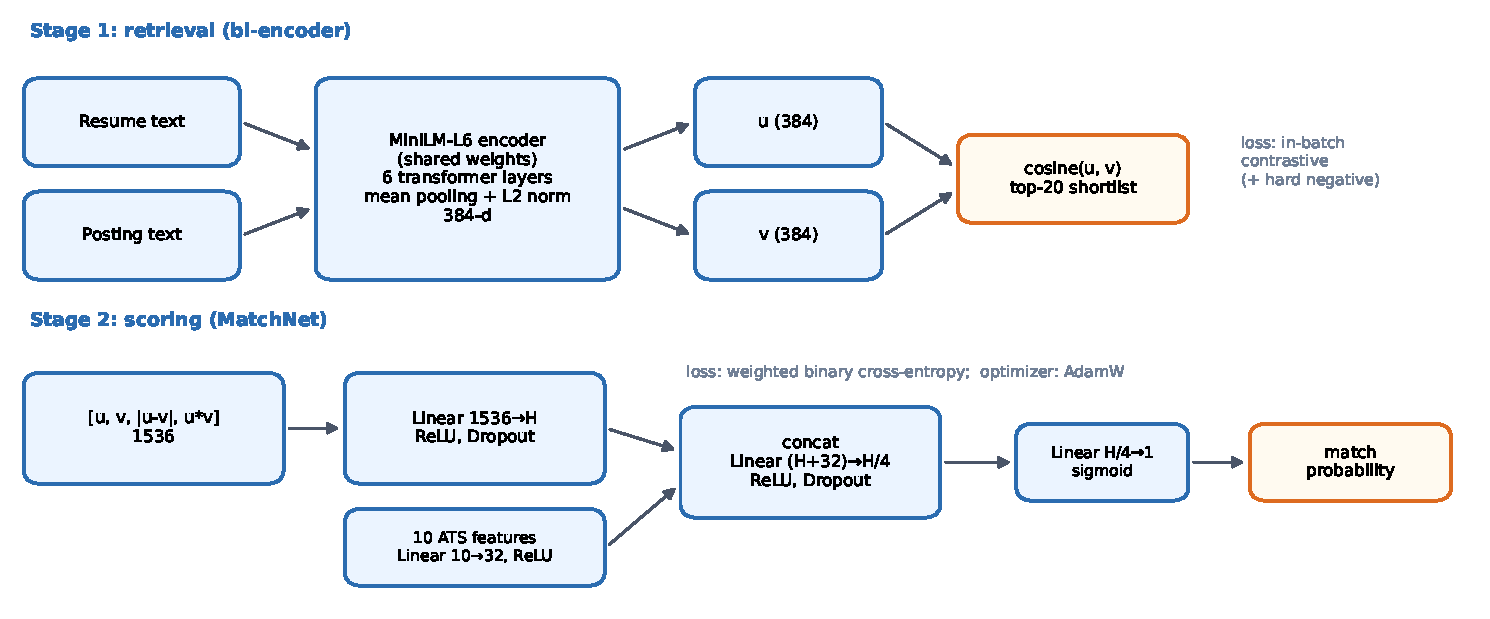
\includegraphics[width=\linewidth]{figures/fig_architecture.pdf}
\caption{Model architecture. Stage~1: the bi-encoder embeds the resume and every open posting and
keeps the 20 closest postings. Stage~2: MatchNet re-scores each shortlisted pair from the two
embeddings and ten scalar features; the top three are returned with their ATS score and apply link.}
\end{figure}

The two-stage design follows the product requirement. Ranking thousands of postings with a model
that reads both documents jointly would be slow, so stage~1 uses independent embeddings that can be
pre-computed for every posting. Stage~2 only sees 20 candidates and can afford richer inputs,
including the explicit skill and experience features that make the result explainable to the user.
Table~\ref{tab:frameworks} lists the frameworks used.

\begin{table}[H]
\centering\small
\begin{tabularx}{\linewidth}{@{}l L@{}}
\toprule
Component & Implementation\\
\midrule
Bi-encoder & PyTorch 2.8 training loop around \code{sentence-transformers} (MiniLM-L6), \code{src/models/bi\_encoder.py}\\
MatchNet & PyTorch \code{nn.Module}, \code{src/models/matchnet.py}\\
Baselines & scikit-learn 1.6 (\code{LogisticRegression}, \code{HistGradientBoostingClassifier}, TF-IDF)\\
Metrics & scikit-learn metrics with bootstrap confidence intervals, \code{src/evaluate.py}\\
Hardware & Apple M1 Pro (16\,GB), PyTorch MPS backend; seed 42 everywhere\\
\bottomrule
\end{tabularx}
\caption{Frameworks and where each component lives in the repository.}\label{tab:frameworks}
\end{table}

\section{Stage 1: Bi-encoder}\label{sec:biencoder}
\paragraph{Layers.} \code{all-MiniLM-L6-v2}: a 6-layer transformer (hidden size 384, 12 attention
heads, 22.7M parameters), inputs truncated to \BiBestLen word pieces, followed by mean pooling over
tokens and L2 normalization. Resumes and postings share the same weights.

\paragraph{Loss.} Multiple-negatives ranking loss. A batch holds $B$ triplets (resume, matching
posting, hard negative posting); hard negatives are postings from a related but different
occupation, mined in Deliverable~1. Each resume must pick its own posting among all $2B$ postings
in the batch, so the other resumes' positives act as additional negatives:
$L = \mathrm{CrossEntropy}(s \cdot \cos(r_i, p_j), \; i)$ with scale $s = 20$.
This uses every posting in the batch as a negative at no extra cost and directly optimizes ranking,
which is what stage~1 is for.

\paragraph{Optimizer.} AdamW (weight decay 0.01), linear warm-up over the first 10\% of steps then
linear decay to zero, gradient-norm clipping at 1.0, gradient checkpointing to fit the 16\,GB
machine. Each epoch draws one triplet per training resume (\BiTriplets triplets), cycling through
that resume's positives and hard negatives across epochs.

\section{Stage 2: MatchNet}\label{sec:matchnet}
\paragraph{Layers.} For resume embedding $u$ and posting embedding $v$ (384-d each, from the
fine-tuned bi-encoder) MatchNet builds the standard interaction vector $[u, v, |u-v|, u \odot v]$
(1,536 values) and passes it through
\begin{itemize}
\item an embedding branch: Linear(1536 $\rightarrow$ $H$), ReLU, Dropout;
\item a feature branch: Linear(10 $\rightarrow$ 32), ReLU, on the standardized scalar features;
\item a head on the concatenation: Linear($H$+32 $\rightarrow$ $H$/4), ReLU, Dropout,
Linear($H$/4 $\rightarrow$ 1), sigmoid.
\end{itemize}
The selected models have $H = \MnAHidden$ (Task~A, \MnAParams parameters) and
$H = \MnBHidden$ (Task~B, \MnBParams parameters).

\paragraph{Loss.} Binary cross-entropy on the logit (\code{BCEWithLogitsLoss}) with
\code{pos\_weight} = negatives / positives in the training split, so that both classes contribute
equally to the gradient despite the class imbalance.

\paragraph{Optimizer.} AdamW (weight decay $10^{-4}$), at most 60 epochs, early stopping when
validation AUC-ROC has not improved for 6 epochs; the weights of the best epoch are restored.

\section{Baselines}
\begin{itemize}
\item \textbf{ATS score (rules)}: the Deliverable~1 score (skill coverage, experience, title and
structure), used as a classifier score directly.
\item \textbf{TF-IDF cosine} and \textbf{MiniLM cosine (pretrained)}: similarity without any training
on our data; \textbf{bi-encoder cosine (fine-tuned)} isolates the gain from stage~1 alone.
\item \textbf{Logistic regression} and \textbf{gradient boosting} (scikit-learn) on the same ten
scalar features plus both cosine similarities, tuned on the validation split. They answer whether a
neural network is needed at all.
\end{itemize}

\section{Hyperparameter Tuning}\label{sec:tuning}
All tuning uses the validation split only; the test split is touched once, for the final numbers.

\paragraph{Bi-encoder.} Fine-tuning a transformer is expensive (about 3~minutes per epoch here),
so instead of a full grid we varied one parameter at a time around the usual sentence-transformer
defaults (learning rate $3\times10^{-5}$, batch 32, length 256): learning rate (three values a
factor of three apart), batch size (which also sets the number of in-batch negatives) and maximum
input length, each for \BiEpochs epochs, \BiRuns runs in total (Table~\ref{tab:bigrid}). The selection criterion is the AUC
of positives against \emph{hard} negatives, because separating related occupations is the difficult
part; random negatives are already easy for the pretrained model.

\begin{table}[H]
\centering\small
\begin{tabularx}{\linewidth}{@{}c c c c r r r r@{}}
\toprule
Learning rate & Batch & Max len & Best ep. & Val AUC & Val AUC (hard) & Val P@3 & Min\\
\midrule
\multicolumn{4}{l}{pretrained MiniLM, no fine-tuning} & 0.644 & 0.539 & 0.429 & --\\
$1\times10^{-5}$ & 32 & 256 & 3 & 0.729 & 0.628 & 0.544 & 8\\
$3\times10^{-5}$ & 32 & 256 & 3 & 0.771 & 0.683 & 0.609 & 8\\
\textbf{$1\times10^{-4}$} & \textbf{32} & \textbf{256} & \textbf{3} & \textbf{0.801} & \textbf{0.724} & \textbf{0.631} & \textbf{8}\\
$3\times10^{-5}$ & 16 & 256 & 3 & 0.793 & 0.714 & 0.629 & 9\\
$3\times10^{-5}$ & 32 & 128 & 3 & 0.751 & 0.666 & 0.579 & 3\\
\bottomrule
\end{tabularx}
\caption{Bi-encoder hyperparameter search (validation split). Selection criterion: AUC of positives vs.\ hard negatives. The selected run is in bold.}\label{tab:bigrid}
\end{table}


The selected configuration (learning rate \BiBestLr, batch \BiBestBs, length \BiBestLen, epoch
\BiBestEpoch) raised validation AUC on hard negatives from \BiPreAucHard to \BiAucHard and
precision@3 from \BiPrePthree to \BiPthree. Three observations justify the choice:
\begin{itemize}
\item \emph{Learning rate} mattered most. With only \BiEpochs epochs, $10^{-5}$ barely moves the
pretrained weights; $10^{-4}$ adapted fastest and showed no sign of damaging the encoder (validation
AUC rose every epoch).
\item \emph{Batch size}: 16 beat 32 at the same learning rate. With a fixed number of epochs, a
smaller batch takes twice as many update steps, which outweighed having fewer in-batch negatives.
\item \emph{Input length}: 128 word pieces is clearly worse than 256 (the median cleaned resume has
\MedWordsRes words, so 128 pieces cut off most of the experience section) and was kept at 256.
\end{itemize}
Every run was still improving at its last epoch, so longer training (and combining
$10^{-4}$ with batch 16) is the obvious next step; it was limited by compute, not by overfitting.

\paragraph{MatchNet.} MatchNet trains in seconds, so we ran a full grid of \MnRuns combinations
per task: learning rate \{$10^{-3}$, $3\times10^{-4}$, $10^{-4}$\}, batch size \{64, 256\}, dropout
\{0.1, 0.3, 0.5\} and hidden size \{128, 256\}. Table~\ref{tab:mngrid} summarizes the effect of each
value; the full grid is in Section~\ref{sec:appendix}.

\begin{table}[H]
\centering\small
\begin{tabularx}{\linewidth}{@{}l c c c@{}}
\toprule
Hyperparameter & Value & Task A: mean / max val AUC & Task B: mean / max val AUC\\
\midrule
Learning rate & $1\times10^{-4}$ & 0.835 / 0.839 & 0.773 / 0.781\\
 & $3\times10^{-4}$ & 0.841 / 0.847 & 0.781 / 0.793\\
 & $1\times10^{-3}$ & \textbf{0.853 / 0.860} & \textbf{0.794 / 0.807}\\
\addlinespace
Batch size & 64 & \textbf{0.845 / 0.860} & \textbf{0.787 / 0.807}\\
 & 256 & 0.840 / 0.857 & 0.779 / 0.800\\
\addlinespace
Dropout & 0.1 & 0.841 / 0.858 & 0.780 / 0.795\\
 & 0.3 & \textbf{0.843 / 0.860} & 0.781 / 0.807\\
 & 0.5 & 0.845 / 0.858 & \textbf{0.788 / 0.807}\\
\addlinespace
Hidden size $H$ & 128 & 0.842 / 0.855 & \textbf{0.784 / 0.807}\\
 & 256 & \textbf{0.844 / 0.860} & 0.782 / 0.806\\
\bottomrule
\end{tabularx}
\caption{MatchNet grid search: all 36 combinations of the values below were trained per task; each cell averages (and maximizes) validation AUC over the runs with that value. Bold marks the value of the selected configuration. The full grid is in the appendix.}\label{tab:mngrid}
\end{table}


Selected: Task~A learning rate \MnALr, batch \MnABs, dropout \MnADrop, $H = \MnAHidden$
(val AUC \MnAValAuc, best epoch \MnAEpoch); Task~B learning rate \MnBLr, batch \MnBBs, dropout
\MnBDrop, $H = \MnBHidden$ (val AUC \MnBValAuc, best epoch \MnBEpoch). The largest learning rate
won on both tasks: with early stopping on validation AUC, a fast optimizer is not at risk of
overfitting, and the network is small. Task~B has only 5,463 training pairs, about half of Task~A,
which is why the smaller network with the strongest dropout was selected there. Batch size
mattered little.

\paragraph{Ablations.} Two questions were checked on the validation split with the selected
configuration. \emph{Does fine-tuning the encoder help MatchNet?} With pretrained instead of
fine-tuned embeddings, validation AUC is \MnAAblPre (Task~A) and \MnBAblPre (Task~B), against
\MnAValAuc and \MnBValAuc. \emph{Do the explicit ATS features help?} Without the feature branch it
is \MnAAblNoFeat (Task~A) and \MnBAblNoFeat (Task~B), so the interpretable features add a small but
consistent gain on top of the embeddings. Fine-tuning helps strongly on Task~A but \emph{not} on
Task~B, where pretrained embeddings are slightly better. The bi-encoder was fine-tuned on Task~A's
occupation labels; it learned to separate occupations, which matters less when most Task~B pairs
already share an occupation and differ in seniority and specific skills. We keep one encoder for
both tasks because the product uses one, and report this as a limitation.

\section{Training Curves}
\begin{figure}[H]
\centering
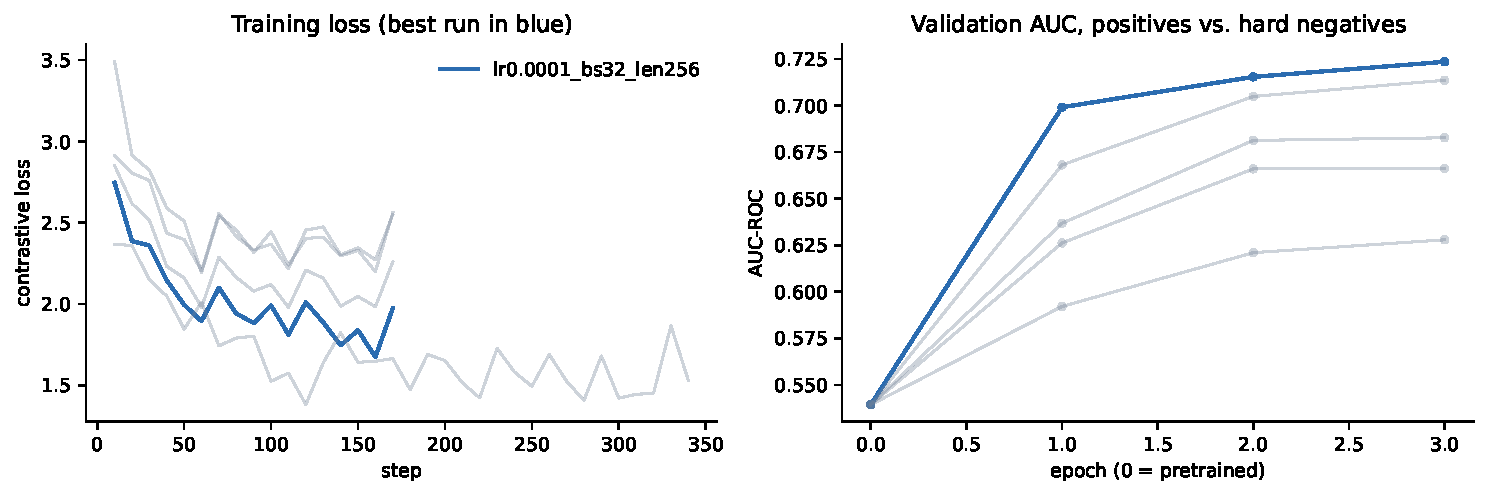
\includegraphics[width=\linewidth]{figures/fig_bi_encoder_curves.pdf}
\caption{Bi-encoder fine-tuning: training loss per 10 steps (left) and validation AUC of positives
vs.\ hard negatives after each epoch (right; epoch 0 is the pretrained model). The selected run is
in blue, the other grid runs in grey.}
\end{figure}

\begin{figure}[H]
\centering
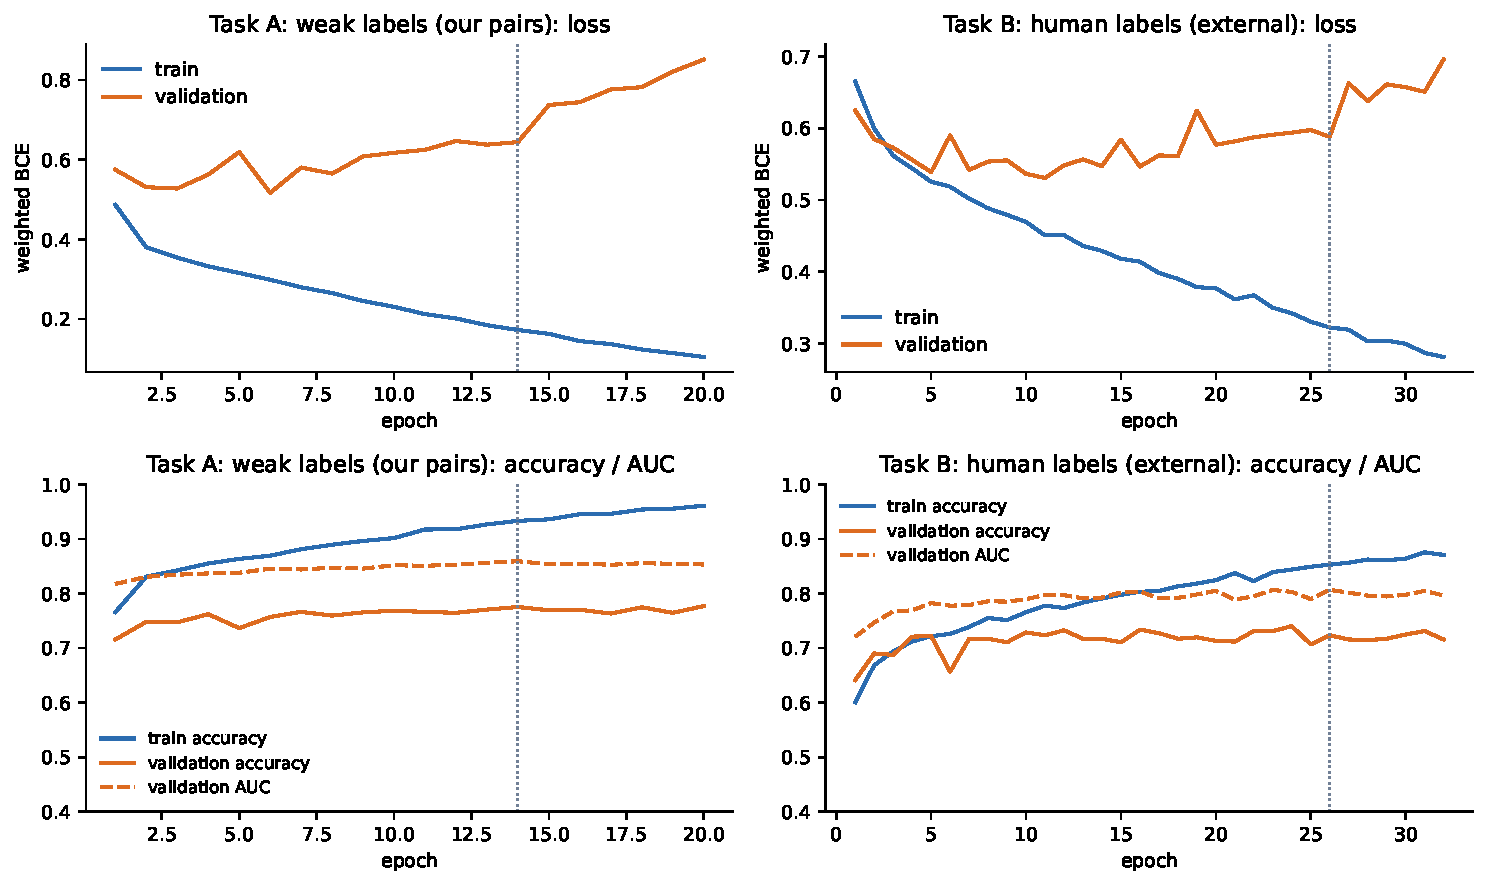
\includegraphics[width=\linewidth]{figures/fig_matchnet_curves.pdf}
\caption{MatchNet training for the selected configurations: loss (top) and accuracy (bottom) on the
training and validation splits. The dashed line marks the early-stopping epoch whose weights are kept.}
\end{figure}

Validation loss starts rising after a few epochs while validation AUC is still flat or improving:
the network keeps ranking pairs correctly but becomes over-confident on the pairs it gets wrong,
which cross-entropy punishes heavily. This is why early stopping monitors AUC, the quantity the
product depends on (ranking), rather than loss; the train--validation gap in accuracy also shows
that dropout and early stopping are needed, since MatchNet can fit the training pairs almost perfectly.

% ---------------------------------------------------------------- Phase 4
\phase{Phase 4: Evaluation \& Analysis}

\section{Validation Strategy}\label{sec:validation}
We use a fixed train / validation / test split rather than K-fold cross-validation. Fine-tuning the
transformer five or ten times per configuration would multiply a one-hour search, and with
thousands of pairs a single held-out split already gives tight confidence intervals (reported
below). The splits are made by \emph{entity}, not by pair, so that no information leaks:
\begin{itemize}
\item \textbf{Task~A}: resumes and postings were assigned to train / validation / test in
Deliverable~1 (70/15/15 by resume, stratified by category); a pair belongs to the split of its
resume and posting. Pairs: \PairsTrain train, \PairsVal validation, \PairsTest test.
\item \textbf{Task~B}: the dataset ships with a train and a test file whose job descriptions are
disjoint. We keep its test file as our test split and carve the validation split out of its train
file by job description (15\% of job descriptions, \code{GroupShuffleSplit}), so validation also
measures generalization to unseen postings.
\end{itemize}
The decision threshold of every model is chosen on the validation split (maximum F1) and applied
unchanged to the test split. 95\% confidence intervals come from 1,000 bootstrap resamples of the
test pairs.

\section{Metrics and Why}\label{sec:metrics}
Both test splits happen to be close to balanced (\ResAPosShare\% and \ResBPosShare\% positive),
but only by construction: in the product, almost every posting is a non-match for a given resume,
so the deployed problem is heavily imbalanced. Accuracy rewards predicting the majority class and
would look good on the deployed problem even for a useless model, so it is reported only for
completeness. We report:
\begin{itemize}
\item \textbf{Precision}: of the postings we recommend, how many are real matches. Low precision
wastes the user's applications and is the product's main failure mode.
\item \textbf{Recall}: of the real matches, how many we find. Low recall hides good jobs.
\item \textbf{F1}: their harmonic mean, the threshold-dependent summary.
\item \textbf{AUC-ROC}: probability that a random positive pair scores above a random negative one.
It is threshold-free and insensitive to class balance, so it is our primary metric for ranking quality.
\item \textbf{PR-AUC} (average precision): complements AUC-ROC when positives are rare, because it
ignores the large pool of easy true negatives.
\end{itemize}
For the product itself we also report \textbf{precision@3}: the share of the three recommended
postings that are relevant.

\section{Results}\label{sec:results}
\begin{table}[H]
\centering\small
\begin{tabularx}{\linewidth}{@{}l r r r r r r@{}}
\toprule
Model & Precision & Recall & F1 & Accuracy & AUC-ROC [95\% CI] & PR-AUC\\
\midrule
ATS score (rules) & 0.498 & 0.997 & 0.665 & 0.500 & 0.588 [0.56, 0.61] & 0.563\\
TF-IDF cosine & 0.552 & 0.973 & 0.704 & 0.594 & 0.571 [0.55, 0.59] & 0.555\\
MiniLM cosine (pretrained) & 0.540 & 0.939 & 0.686 & 0.574 & 0.661 [0.64, 0.68] & 0.622\\
Bi-encoder cosine (fine-tuned) & 0.639 & 0.876 & 0.739 & 0.694 & 0.790 [0.77, 0.81] & 0.770\\
Logistic regression & 0.659 & 0.864 & 0.748 & 0.711 & 0.808 [0.79, 0.82] & 0.791\\
Gradient boosting & 0.724 & 0.810 & 0.764 & 0.752 & 0.832 [0.82, 0.85] & 0.818\\
\textbf{MatchNet} & \textbf{0.705} & \textbf{0.883} & \textbf{0.784} & \textbf{0.759} & \textbf{0.862 [0.85, 0.88]} & \textbf{0.855}\\
\bottomrule
\end{tabularx}
\caption{Task A (weak labels): test-set results (n = 2,352, 50\% positive). Thresholds were chosen on the validation split by maximum F1.}\label{tab:resweak}
\end{table}

\begin{table}[H]
\centering\small
\begin{tabularx}{\linewidth}{@{}l r r r r r r@{}}
\toprule
Model & Precision & Recall & F1 & Accuracy & AUC-ROC [95\% CI] & PR-AUC\\
\midrule
ATS score (rules) & 0.514 & 0.997 & 0.678 & 0.516 & 0.536 [0.51, 0.56] & 0.544\\
TF-IDF cosine & 0.574 & 0.784 & 0.663 & 0.591 & 0.612 [0.58, 0.64] & 0.582\\
MiniLM cosine (pretrained) & 0.537 & 0.876 & 0.666 & 0.550 & 0.579 [0.55, 0.61] & 0.592\\
Bi-encoder cosine (fine-tuned) & 0.571 & 0.887 & 0.695 & 0.601 & 0.633 [0.61, 0.66] & 0.607\\
Logistic regression & 0.563 & 0.897 & 0.692 & 0.590 & 0.648 [0.62, 0.67] & 0.622\\
Gradient boosting & 0.594 & 0.876 & 0.708 & 0.630 & 0.695 [0.67, 0.72] & 0.679\\
\textbf{MatchNet} & \textbf{0.668} & \textbf{0.822} & \textbf{0.737} & \textbf{0.699} & \textbf{0.768 [0.74, 0.79]} & \textbf{0.757}\\
\bottomrule
\end{tabularx}
\caption{Task B (human labels): test-set results (n = 1,759, 51\% positive). Thresholds were chosen on the validation split by maximum F1.}\label{tab:reshuman}
\end{table}


\paragraph{Task A.} MatchNet reaches F1 \ResAF and AUC-ROC \ResAAuc (95\% CI \ResAAucLo--\ResAAucHi)
on \ResAN test pairs, against \ResAAtsAuc for the rule-based ATS score, \ResAPreAuc for the
pretrained encoder and \ResABiAuc for the fine-tuned bi-encoder alone. Accuracy by pair type:
\AccPos on positives, \AccRand on random negatives, but only \AccHard on hard negatives. Almost all
remaining errors are postings from a related occupation that the model accepts; this is the main
weakness and the focus of the error analysis.

\paragraph{Task B.} On human labels MatchNet reaches F1 \ResBF (precision \ResBP, recall \ResBR) and
AUC-ROC \ResBAuc (95\% CI \ResBAucLo--\ResBAucHi), against \ResBAtsAuc for the ATS score and
\ResBPreAuc for the pretrained encoder. Its mean score rises with the human grade: \FitNo for No~Fit,
\FitPot for Potential~Fit and \FitGood for Good~Fit; separating Good from No Fit alone gives AUC
\AucGoodNo. The model therefore separates No~Fit from the rest well but barely distinguishes
Potential from Good~Fit. The rule-based ATS score is close to chance on both tasks
(AUC \ResAAtsAuc and \ResBAtsAuc): it accepts nearly everything (recall above 0.99), which shows why
a learned model is needed. Gradient boosting on the same features is the strongest baseline; MatchNet
beats it on every threshold-free metric.

\begin{figure}[H]
\centering
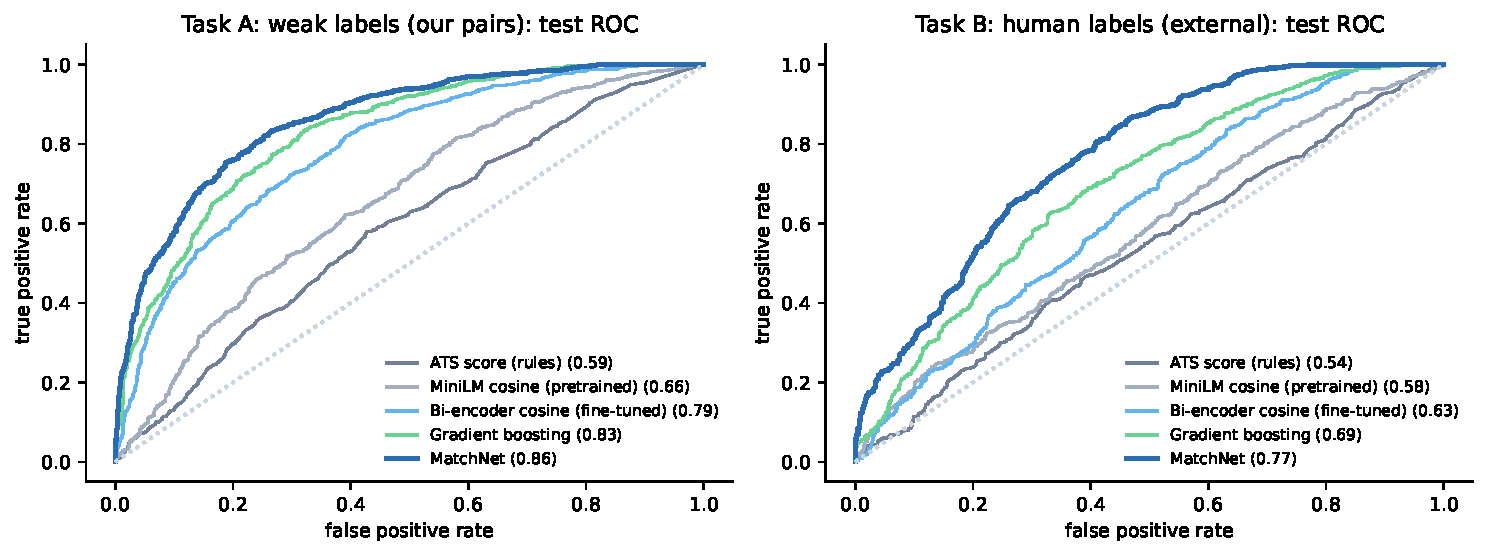
\includegraphics[width=\linewidth]{figures/fig_roc.pdf}
\caption{ROC curves on the test splits of Task~A (left) and Task~B (right).}
\end{figure}

\begin{figure}[H]
\centering
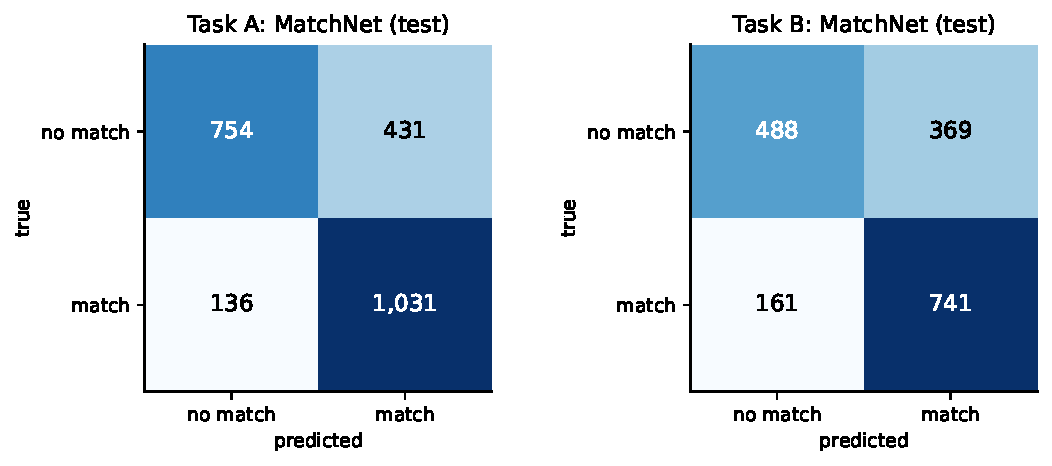
\includegraphics[width=0.8\linewidth]{figures/fig_confusion.pdf}
\caption{MatchNet confusion matrices on the test splits at the validation-selected threshold.}
\end{figure}

\paragraph{Top-3 recommendation.} Table~\ref{tab:retrieval} evaluates the product flow end to end:
for each test resume, all test postings are ranked and the top three are checked.

\begin{table}[H]
\centering\small
\begin{tabularx}{\linewidth}{@{}L r@{}}
\toprule
Ranker & Precision@3\\
\midrule
TF-IDF cosine & 0.406\\
MiniLM (pretrained) & 0.417\\
Bi-encoder (fine-tuned) & 0.634\\
Bi-encoder + MatchNet re-rank & 0.641\\
Random ranking (expected) & 0.050\\
\bottomrule
\end{tabularx}
\caption{Top-3 recommendation on the test split: 395 resumes, each ranked against all 2,565 test postings with a known occupation. A recommended posting counts as relevant if it belongs to the resume's occupation.}\label{tab:retrieval}
\end{table}


Fine-tuning lifts precision@3 from \PthreePre (pretrained) to \PthreeFt, so roughly two of the
three recommended postings are in the right occupation, against one in twenty for a random ranking
(\PthreeRandom). Re-ranking the top 20 with MatchNet adds only a little (\PthreeRerank) on this
occupation-level criterion; its value is in a match score that also weighs skills and experience, and in the
explicit skill features shown to the user. The weakest occupations are \PthreeWorst;
the strongest are \PthreeBest.

\section{Error Analysis}\label{sec:errors}
\emph{Owner: Muaaz Fahad, module \code{src/error\_analysis.py}.}

The error analysis breaks MatchNet's test errors down by resume category, pair type and human fit
grade, compares the features of correct and incorrect predictions, and inspects the most confident
mistakes (Table~\ref{tab:errcat}).

\begin{table}[H]
\centering\small
\begin{tabularx}{\linewidth}{@{}L r r r r@{}}
\toprule
Resume category & Precision & Recall & F1 & Pairs\\
\midrule
\multicolumn{5}{l}{\emph{Pending: run} \code{src/error\_analysis.py}}\\
\bottomrule
\end{tabularx}
\caption{MatchNet per resume category on the Task A test split.}\label{tab:errcat}
\end{table}


\begin{itemize}
\item Worst categories by F1: \ErrWorst. Best: \ErrBest.
\item Task~A error rate by pair type: positives \ErrPos, hard negatives \ErrHard, random negatives \ErrRand.
\item Task~B error rate by human grade: No~Fit \ErrNoFit, Potential~Fit \ErrPot, Good~Fit \ErrGood.
\item False positives / false negatives on Task~A: \ResAFP / \ResAFN; on Task~B: \ResBFP / \ResBFN.
\end{itemize}

\section{Bias Check}\label{sec:bias}
\emph{Owner: Hanan Ishaque, module \code{src/bias\_check.py}.}

A matcher must not change its decision because of who the candidate is. We test this
counterfactually: for \BiasN test pairs we create resume variants that differ in \emph{one}
attribute only and measure how much the MatchNet score moves. The resumes were anonymized in
Deliverable~1, so the attribute is re-inserted explicitly:
\begin{itemize}
\item \textbf{gender (name)}: a male vs.\ a female first name with the same surname;
\item \textbf{origin (name)}: a Pakistani vs.\ a Western name;
\item \textbf{university}: a top-ranked vs.\ a less prestigious university with the same degree;
\item \textbf{gender (pronouns)}: he/his/him vs.\ she/her/her in the body text.
\end{itemize}
Several name pairs are averaged per test. For each test we report the mean paired score difference
with a bootstrap 95\% interval, a Wilcoxon signed-rank test, and the share of pairs whose
accept/reject decision flips at the MatchNet threshold (Table~\ref{tab:bias}).

\begin{table}[H]
\centering\small
\begin{tabularx}{\linewidth}{@{}L r r r r r@{}}
\toprule
Counterfactual test & Mean $\Delta$ & 95\% CI & Mean $|\Delta|$ & $p$ & Decisions flipped\\
\midrule
gender name & +0.0096 & [+0.0069, +0.0128] & 0.0149 & $<0.001$ & 0.7\%\\
origin name & -0.0142 & [-0.0207, -0.0078] & 0.0274 & $<0.001$ & 1.7\%\\
university & +0.0000 & [-0.0064, +0.0062] & 0.0250 & 0.765 & 1.3\%\\
gender pronoun & +0.0000 & [-0.0000, +0.0001] & 0.0001 & 0.086 & 0.0\%\\
\bottomrule
\end{tabularx}
\caption{Bias check: change in MatchNet score when only one attribute of the resume is swapped (variant B minus variant A).}\label{tab:bias}
\end{table}


Conclusion: \BiasConclusion

% ---------------------------------------------------------------- wrap-up
\section{Limitations}
\begin{itemize}
\item Task~A labels are occupation-level, so Task~A scores overstate how well the model judges
seniority or specific skills; Task~B is the more honest number but is a single external dataset.
\item In Task~B, test job descriptions are unseen but almost all test resumes also appear (with
other postings) in training, so it measures generalization to new postings rather than new candidates.
\item The bi-encoder was fine-tuned on occupation labels, which does not help human fit judgements
(Section~\ref{sec:tuning}); fine-tuning on graded fit labels is future work.
\item MatchNet accepts too many postings from related occupations (hard negatives, Section~\ref{sec:results}).
\item Inputs are truncated to \BiBestLen word pieces; long resumes lose their later sections.
\item Most live postings collected for Deliverable~1 have since expired; the pool must be refreshed
(\code{make refresh}) before a demo.
\end{itemize}

\section{Reproducibility and Model Weights}\label{sec:repro}
Code is in \code{src/} (models in \code{src/models/}), dependencies in \code{requirements.txt}.
Weights are not stored in Git; they are published on the Hugging Face Hub and linked from the
README (\code{huggingface.co/Suf-7/resumatch-models}), or rebuilt from scratch with:
\begin{itemize}
\item \code{make train} --- bi-encoder grid search, pair matrices, MatchNet grid search;
\item \code{make evaluate} --- test metrics, top-3 retrieval, figures, report tables;
\item \code{make report2} --- this PDF.
\end{itemize}

\section{Contribution Table}\label{sec:contrib}
Table~\ref{tab:contrib} is generated from \code{git log}, so it reflects the commit history exactly.

\begin{table}[H]
\centering\small
\begin{tabularx}{\linewidth}{@{}l r r L@{}}
\toprule
Git author & Commits & Lines & Main modules (by lines changed)\\
\midrule
Muhammad Sufyan & 7 & +4,857 / $-$46 & \code{report (build\_pdf.py)}, \code{build\_features.py}, \code{scrape\_jobs.py}, \code{common.py}, \code{report (make\_tables.py)}\\
Muaaz Fahad & 0 & +0 / $-$0 & ---\\
Hanan Ishaque & 0 & +0 / $-$0 & ---\\
\bottomrule
\end{tabularx}
\caption{Contribution table generated from the Git history by \code{report/contributions.py} (generated files such as figures, PDFs and JSON statistics are excluded).}\label{tab:contrib}
\end{table}


\begin{table}[H]
\centering\small
\begin{tabularx}{\linewidth}{@{}l L@{}}
\toprule
Member & Deliverable 2 responsibility\\
\midrule
Muhammad Sufyan & Bi-encoder and MatchNet implementation, training and tuning, baselines, evaluation, retrieval evaluation, figures, report\\
Muaaz Fahad & Error analysis (\code{src/error\_analysis.py}), Section~\ref{sec:errors}\\
Hanan Ishaque & Bias check (\code{src/bias\_check.py}), Section~\ref{sec:bias}\\
\bottomrule
\end{tabularx}
\caption{Module ownership.}
\end{table}

\clearpage
\section{Appendix: Full MatchNet Grid}\label{sec:appendix}
\begin{table}[H]
\centering\footnotesize
\begin{tabularx}{\linewidth}{@{}c c c c r r r r@{}}
\toprule
LR & Batch & Dropout & $H$ & A: val AUC & A: epoch & B: val AUC & B: epoch\\
\midrule
$1\times10^{-3}$ & 64 & 0.1 & 128 & 0.852 & 14 & 0.793 & 20\\
$1\times10^{-3}$ & 64 & 0.1 & 256 & 0.858 & 14 & 0.795 & 14\\
$1\times10^{-3}$ & 64 & 0.3 & 128 & 0.851 & 16 & 0.807 & 23\\
$1\times10^{-3}$ & 64 & 0.3 & 256 & 0.860 & 14 & 0.796 & 11\\
$1\times10^{-3}$ & 64 & 0.5 & 128 & 0.855 & 23 & 0.807 & 26\\
$1\times10^{-3}$ & 64 & 0.5 & 256 & 0.858 & 14 & 0.806 & 14\\
$1\times10^{-3}$ & 256 & 0.1 & 128 & 0.847 & 29 & 0.782 & 11\\
$1\times10^{-3}$ & 256 & 0.1 & 256 & 0.846 & 30 & 0.780 & 9\\
$1\times10^{-3}$ & 256 & 0.3 & 128 & 0.847 & 31 & 0.786 & 18\\
$1\times10^{-3}$ & 256 & 0.3 & 256 & 0.853 & 31 & 0.789 & 16\\
$1\times10^{-3}$ & 256 & 0.5 & 128 & 0.850 & 31 & 0.800 & 26\\
$1\times10^{-3}$ & 256 & 0.5 & 256 & 0.857 & 38 & 0.793 & 16\\
$3\times10^{-4}$ & 64 & 0.1 & 128 & 0.841 & 31 & 0.785 & 16\\
$3\times10^{-4}$ & 64 & 0.1 & 256 & 0.843 & 31 & 0.779 & 16\\
$3\times10^{-4}$ & 64 & 0.3 & 128 & 0.841 & 27 & 0.783 & 23\\
$3\times10^{-4}$ & 64 & 0.3 & 256 & 0.845 & 31 & 0.778 & 16\\
$3\times10^{-4}$ & 64 & 0.5 & 128 & 0.844 & 31 & 0.793 & 34\\
$3\times10^{-4}$ & 64 & 0.5 & 256 & 0.847 & 36 & 0.787 & 16\\
$3\times10^{-4}$ & 256 & 0.1 & 128 & 0.836 & 59 & 0.778 & 20\\
$3\times10^{-4}$ & 256 & 0.1 & 256 & 0.837 & 46 & 0.770 & 20\\
$3\times10^{-4}$ & 256 & 0.3 & 128 & 0.839 & 40 & 0.772 & 32\\
$3\times10^{-4}$ & 256 & 0.3 & 256 & 0.838 & 37 & 0.771 & 26\\
$3\times10^{-4}$ & 256 & 0.5 & 128 & 0.841 & 59 & 0.786 & 50\\
$3\times10^{-4}$ & 256 & 0.5 & 256 & 0.840 & 38 & 0.784 & 44\\
$1\times10^{-4}$ & 64 & 0.1 & 128 & 0.836 & 58 & 0.776 & 31\\
$1\times10^{-4}$ & 64 & 0.1 & 256 & 0.836 & 51 & 0.773 & 20\\
$1\times10^{-4}$ & 64 & 0.3 & 128 & 0.836 & 51 & 0.772 & 34\\
$1\times10^{-4}$ & 64 & 0.3 & 256 & 0.837 & 40 & 0.773 & 25\\
$1\times10^{-4}$ & 64 & 0.5 & 128 & 0.839 & 59 & 0.774 & 35\\
$1\times10^{-4}$ & 64 & 0.5 & 256 & 0.838 & 40 & 0.781 & 52\\
$1\times10^{-4}$ & 256 & 0.1 & 128 & 0.831 & 59 & 0.777 & 51\\
$1\times10^{-4}$ & 256 & 0.1 & 256 & 0.831 & 59 & 0.773 & 38\\
$1\times10^{-4}$ & 256 & 0.3 & 128 & 0.832 & 60 & 0.771 & 55\\
$1\times10^{-4}$ & 256 & 0.3 & 256 & 0.833 & 59 & 0.771 & 38\\
$1\times10^{-4}$ & 256 & 0.5 & 128 & 0.833 & 60 & 0.767 & 59\\
$1\times10^{-4}$ & 256 & 0.5 & 256 & 0.835 & 59 & 0.774 & 51\\
\bottomrule
\end{tabularx}
\caption{Full MatchNet grid (validation AUC and early-stopped epoch per task).}\label{tab:mnfull}
\end{table}


\end{document}
